\documentclass[../main.tex]{subfiles}

\begin{document}
\section{Results}\label{sec:results}
\subsection{The $L=2$ case}
\Cref{tab:L2-numerical-vs-analytical} shows a number of selected expectation values for the energy, specific heat capacity, mean absolute magnetization and magnetic susceptibility. From the table it is evident that the selected expectation values converges to the analytical values, and that it is necessary to have approximately $10^6$ cycles to get the best estimates. 

\begin{table}[!htb]
\caption{Computed thermodynamic quantities for several Monte Carlo cycles per spin with $L=2$ and $T=1$ starting from an ordered spin configuration.} 
\begin{center}
\begin{tabular}{ c c c c c}
\toprule
Cycles & \ensuremath{\braket{E}/L^2} & \ensuremath{\braket{|M|}/L^2} & \ensuremath{C_v/L^2} & \ensuremath{\chi/L^2} \\
\midrule
$10^2$ & -1.8800 & 0.9650 & 0.9024 & 0.2379\\
$10^3$ & -1.9880 & 0.9950 & 0.0954 & 0.0259\\
$10^4$ & -1.9964 & 0.9987 & 0.0287 & 3.9656\\
$10^5$ & -1.9957 & 0.9986 & 0.0346 & 3.9894\\
$10^6$ & -1.9962 & 0.9987 & 0.0305 & 3.9910\\

\midrule
Analytical & -1.9960 & 0.9987 & 0.0321 & 3.9933 \\
\bottomrule
\end{tabular}
\end{center}
\label{tab:L2-numerical-vs-analytical}
\end{table}

\subsection{Estimation of equilibration time}
\label{subsec:equilibration-time}
%An estimate of the equilibration time was found for a system with $L=20$. 

In \cref{fig:equilibration-time} we plot the four thermodynamic expectation values of energy, absolute magnetization, heat capacity and magnetic susceptibility, as running expectation values over the number of MC cycles. They are plotted for the case of the initial state being the ground state where all spins point in the same direction, and secondly for a randomized initial spin state.

\begin{figure}[htb!]
    \centering
    \begin{subfigure}[b]{\textwidth}
    \centering
    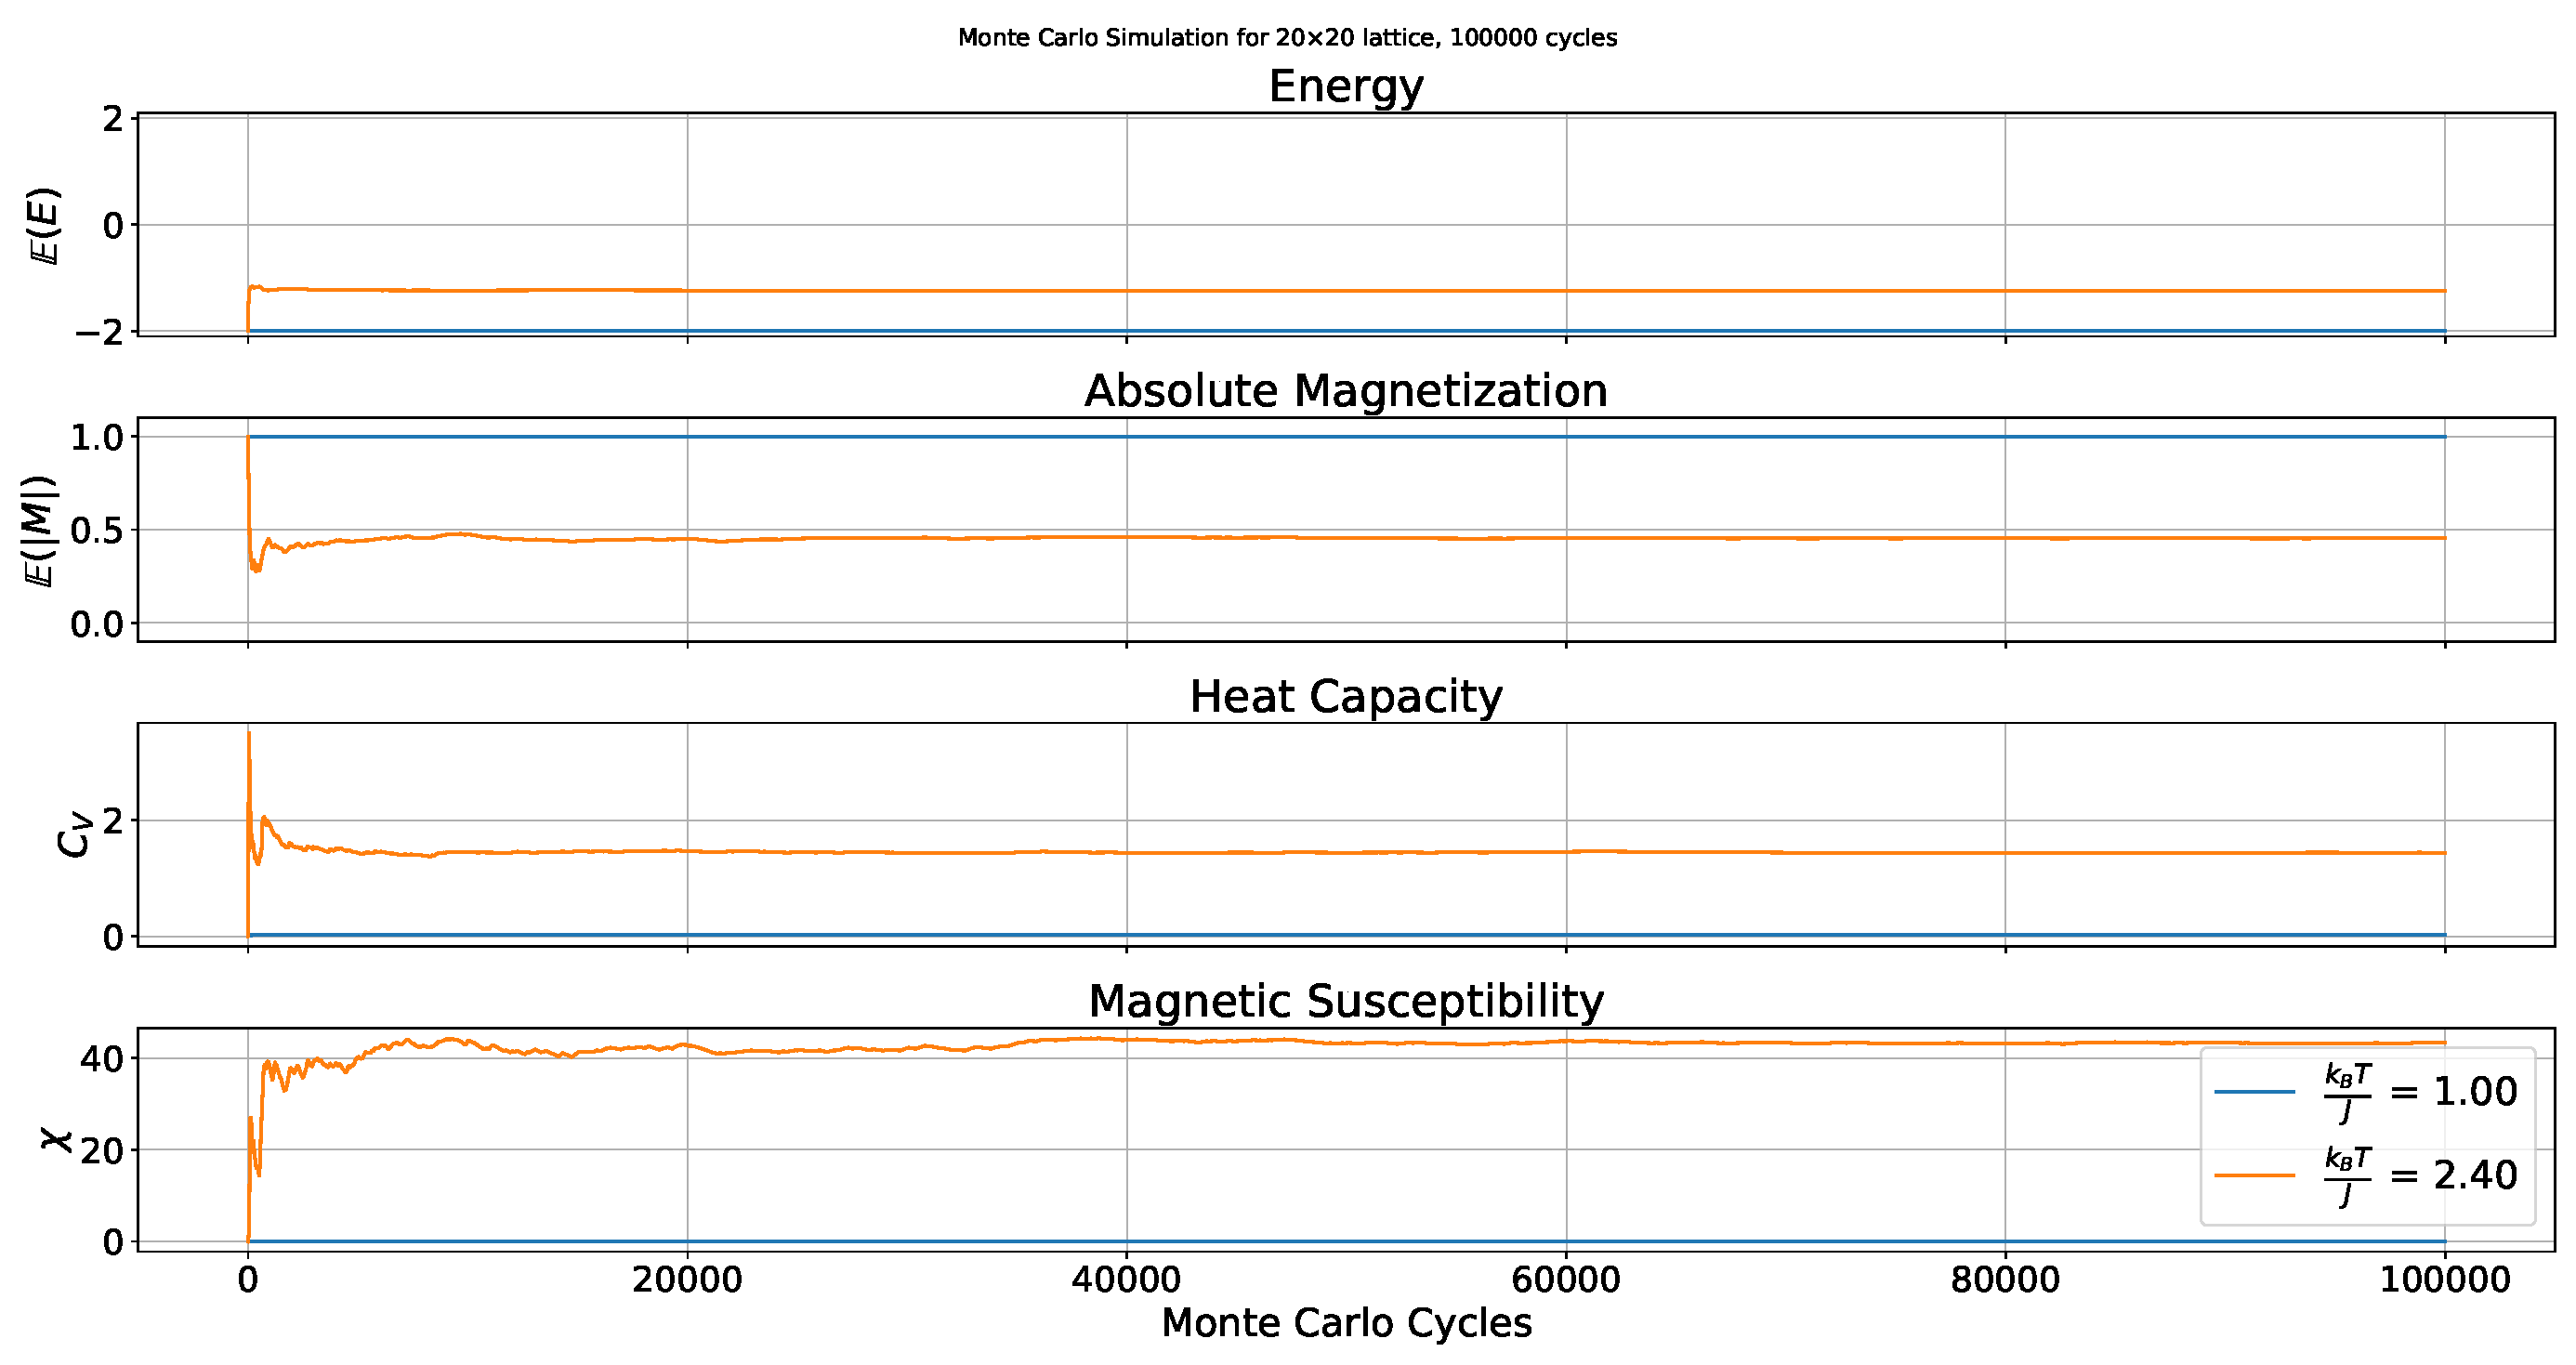
\includegraphics[trim=0.cm 0.cm 0.cm 1.cm, clip,width=1.0\textwidth]{../figures/MC_ising_20x20_1E5_cycles_T_1.0_2.4_rng_0.pdf}
    \caption{Starting from the ground state.}
    \label{fig:equilibration-time-no-rng}
    \end{subfigure}
    
    \begin{subfigure}[b]{\textwidth}
    \centering
    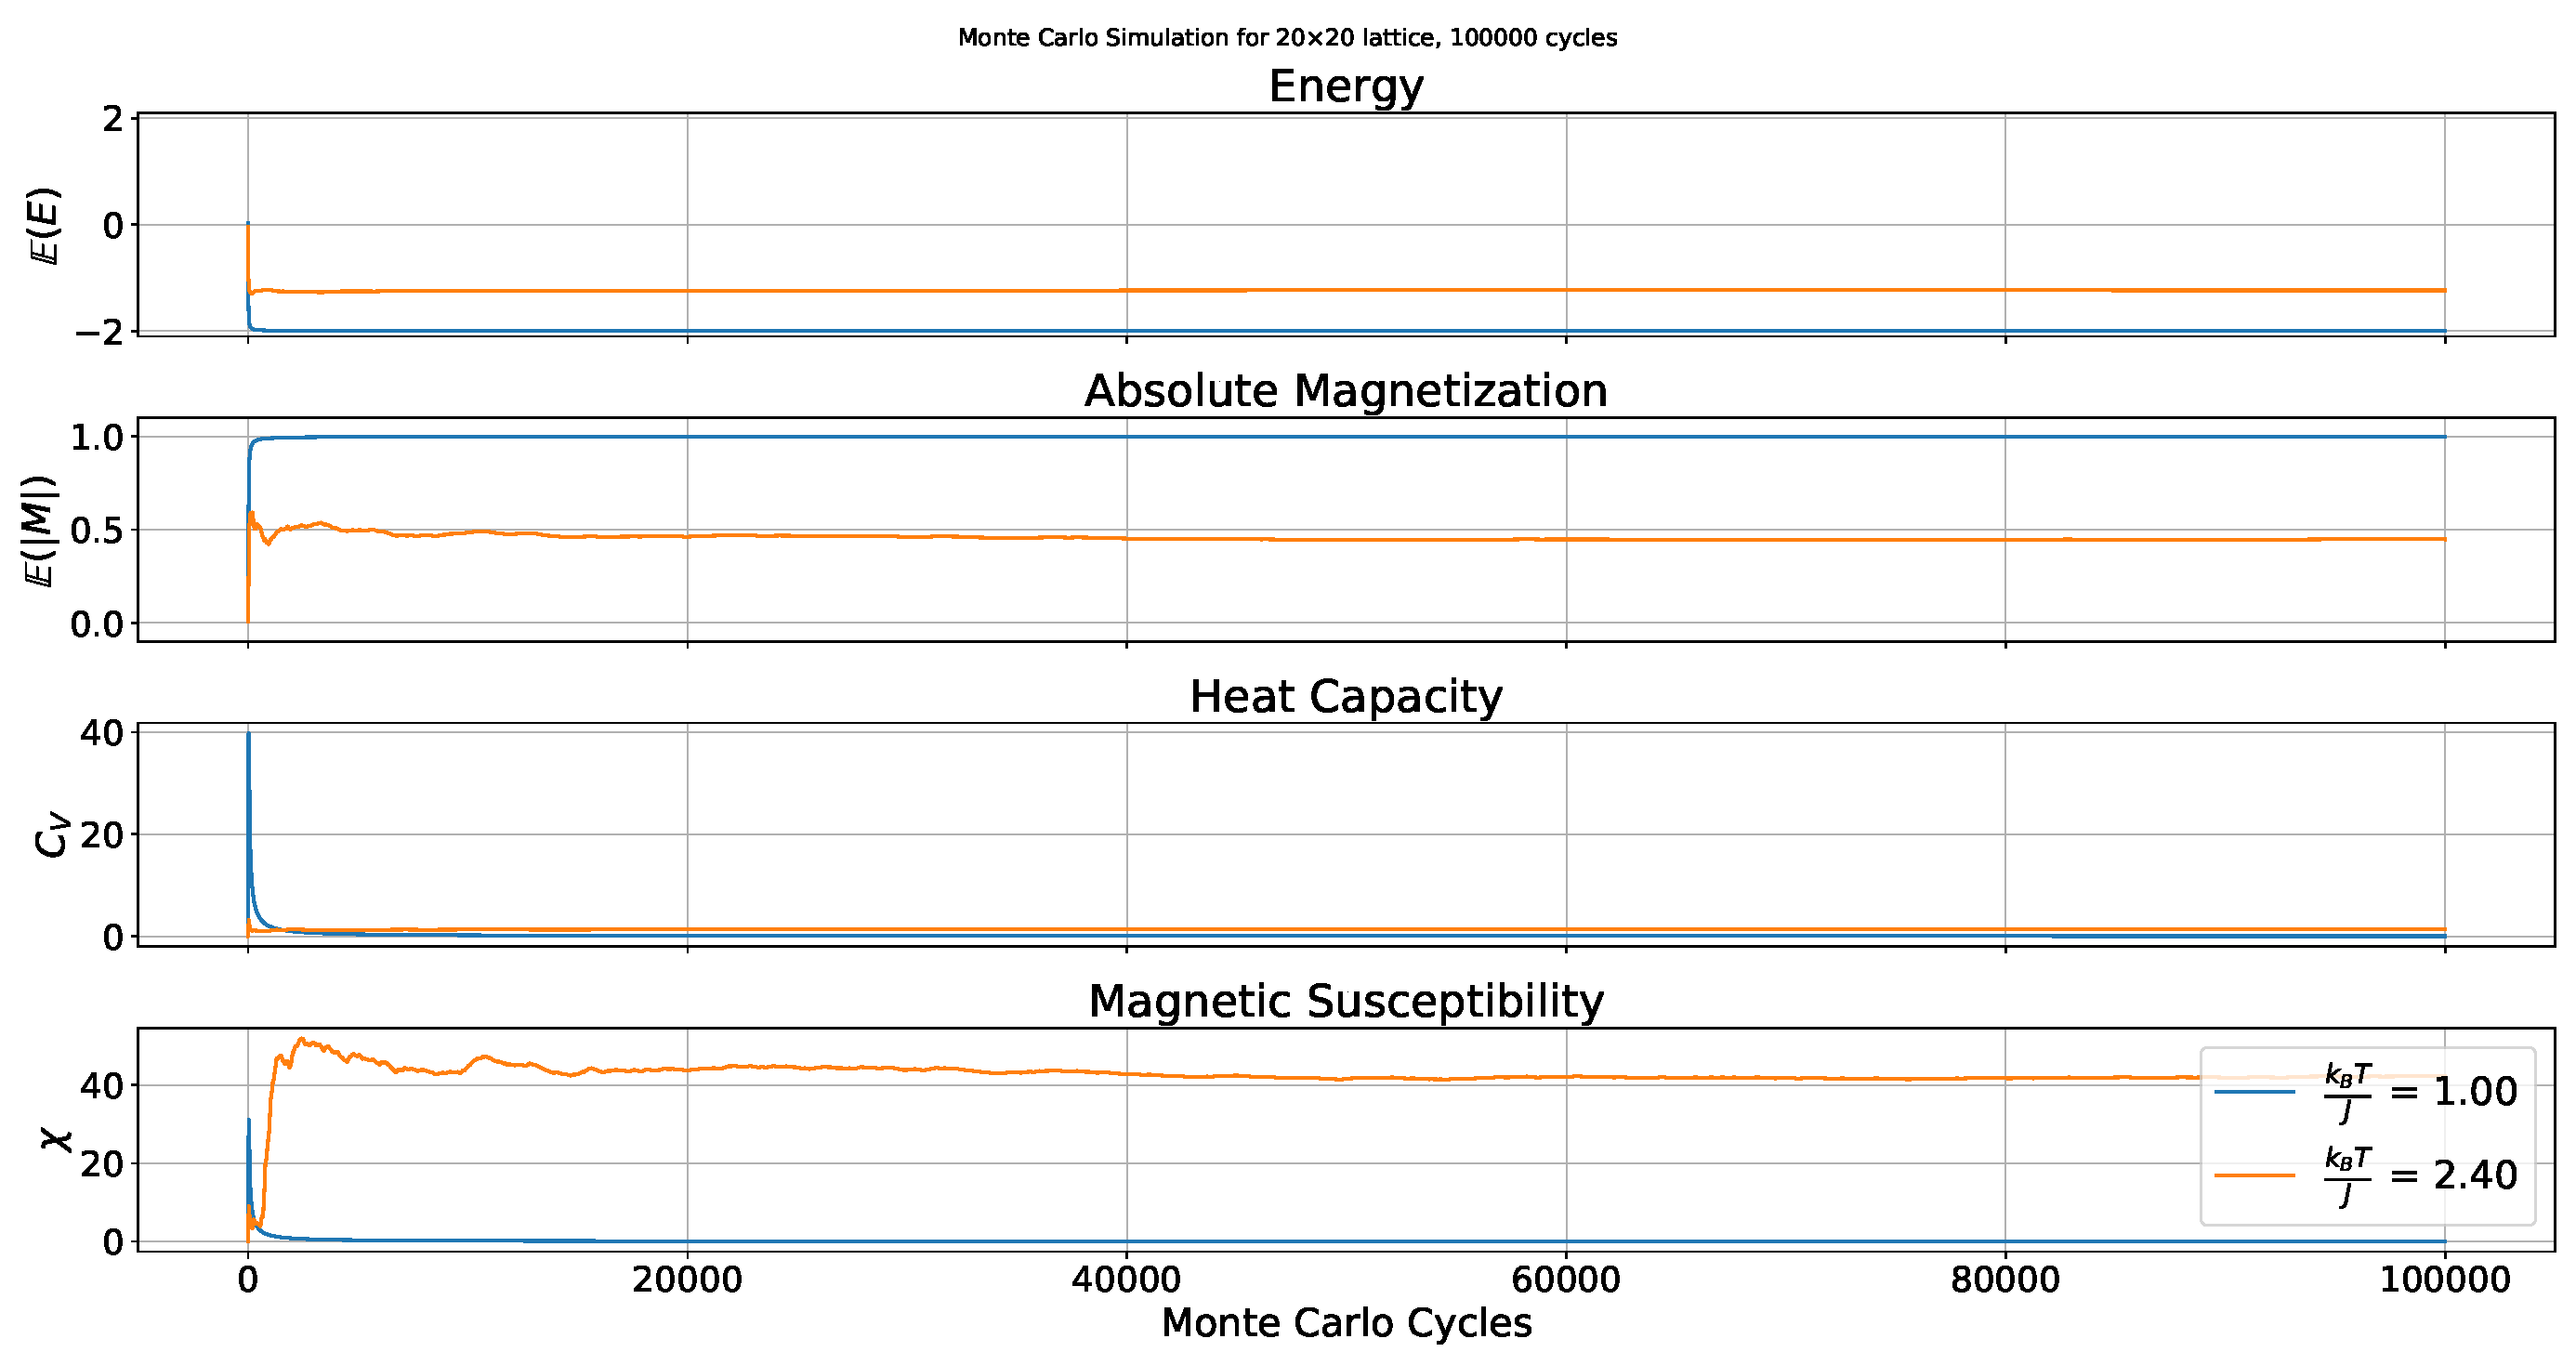
\includegraphics[trim=0.cm 0.cm 0.cm 1.cm, clip,width=1.0\textwidth]{../figures/MC_ising_20x20_1E5_cycles_T_1.0_2.4_rng_1.pdf}
    \caption{Starting from a randomized state.}
    \label{fig:equilibration-time-rng}
    \end{subfigure}
    \caption{Thermodynamic expectation values per spin as a function of Monte Carlo cycles. The system is a $20 \times 20$ lattice, for two temperatures $\frac{k_B T}{J} = \{1.0, 2.4\}$. The different thermodynamic quantities have slightly different equilibration times, but most notably is the temperature dependence. The system begins in the ground state with all spins pointing in the same direction.}
    \label{fig:equilibration-time}
\end{figure}

\newpage

\subsection{Accepted spin-flips}
To find the number of accepted spin configurations, we plot the number of accepted spin flips for select temperatures as a function of Monte Carlo cycles in \cref{fig:spin-flips}. As explained in \cref{subsec:metropolis}, there will be more potential spin flips than Monte Carlo cycles. 

\begin{figure}[htb!]
    \centering
    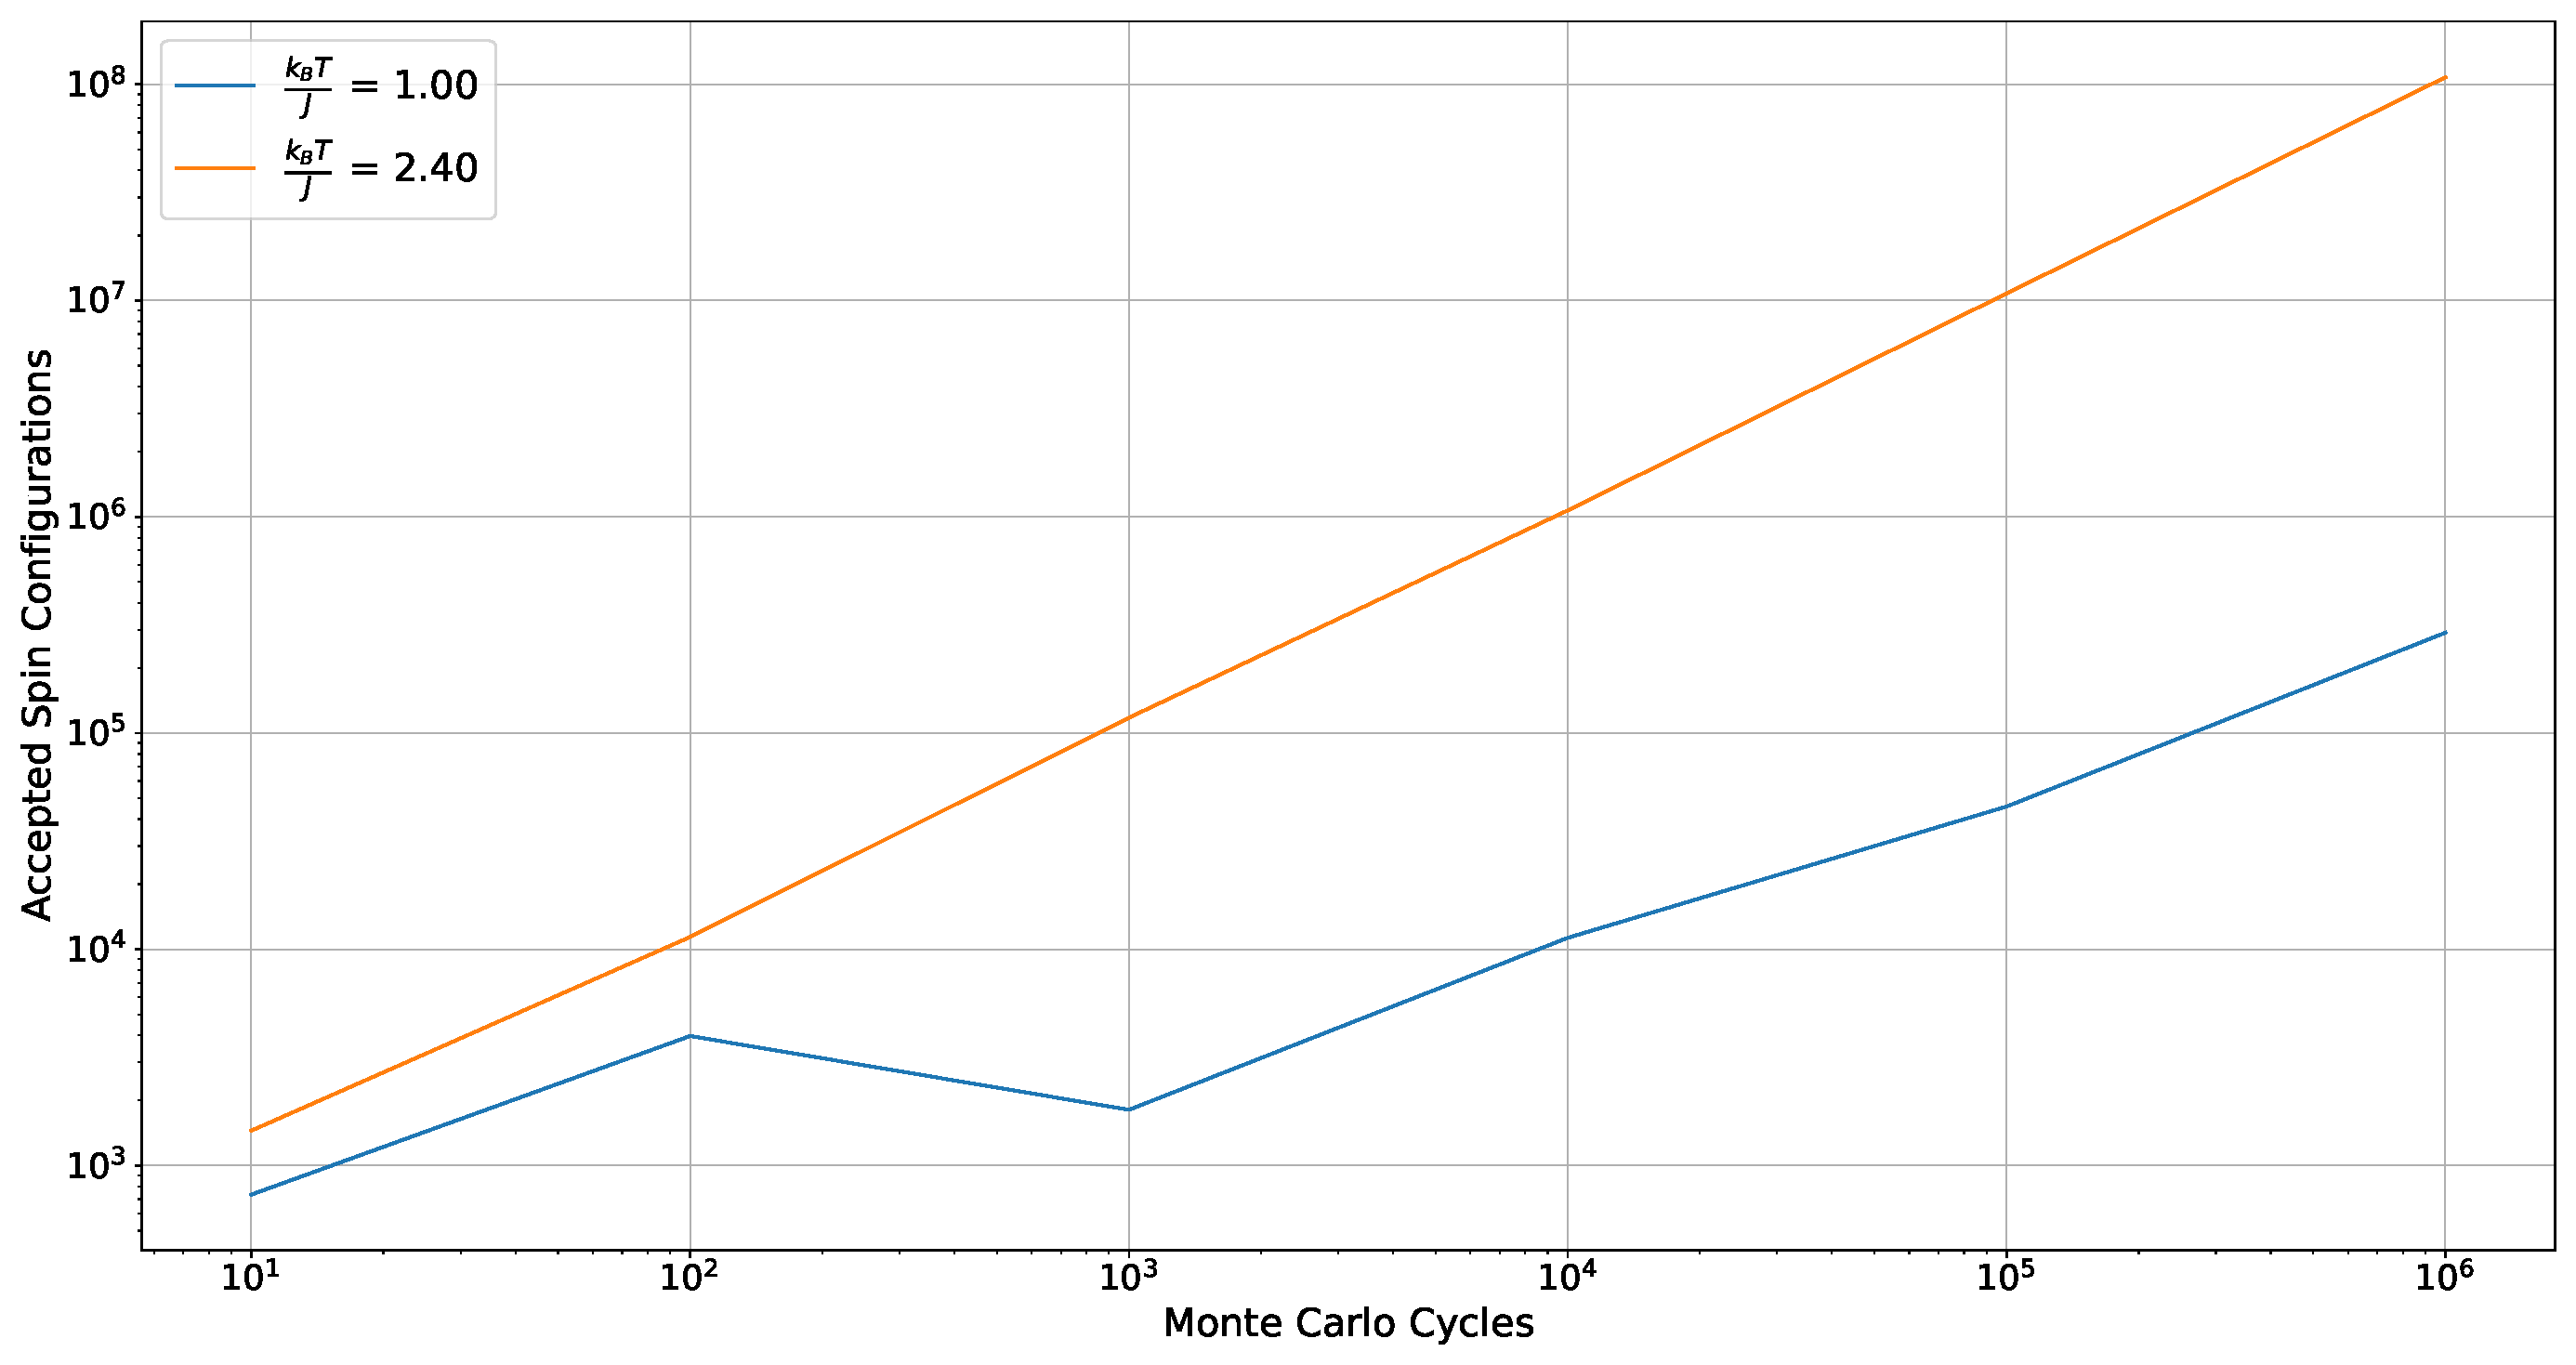
\includegraphics[trim=0.cm 0.cm 0.cm 0.cm, clip,width=1.0\textwidth]{../figures/spin_flips_ising_20x20_1E6_cycles_T_1.0_2.4_rng_1.pdf}
    \caption{Number of accepted spin-flips as a function of Monte Carlo cycles. The system is a $20 \times 20$ lattice starting from a random configuration, and since each Monte Carlo cycle involves up to $20 \times 20 = 400$ spin flips, the number of spin flips tends to be higher than the number of cycles. We see a mostly linear relationship, while the lower temperature accepts fewer spin flips. }
    \label{fig:spin-flips}
\end{figure}

We also studied the number of accepted spin-flips as a function of temperature, plotted in \cref{fig:spin-flips-temp}. 

\begin{figure}[htb!]
    \centering
    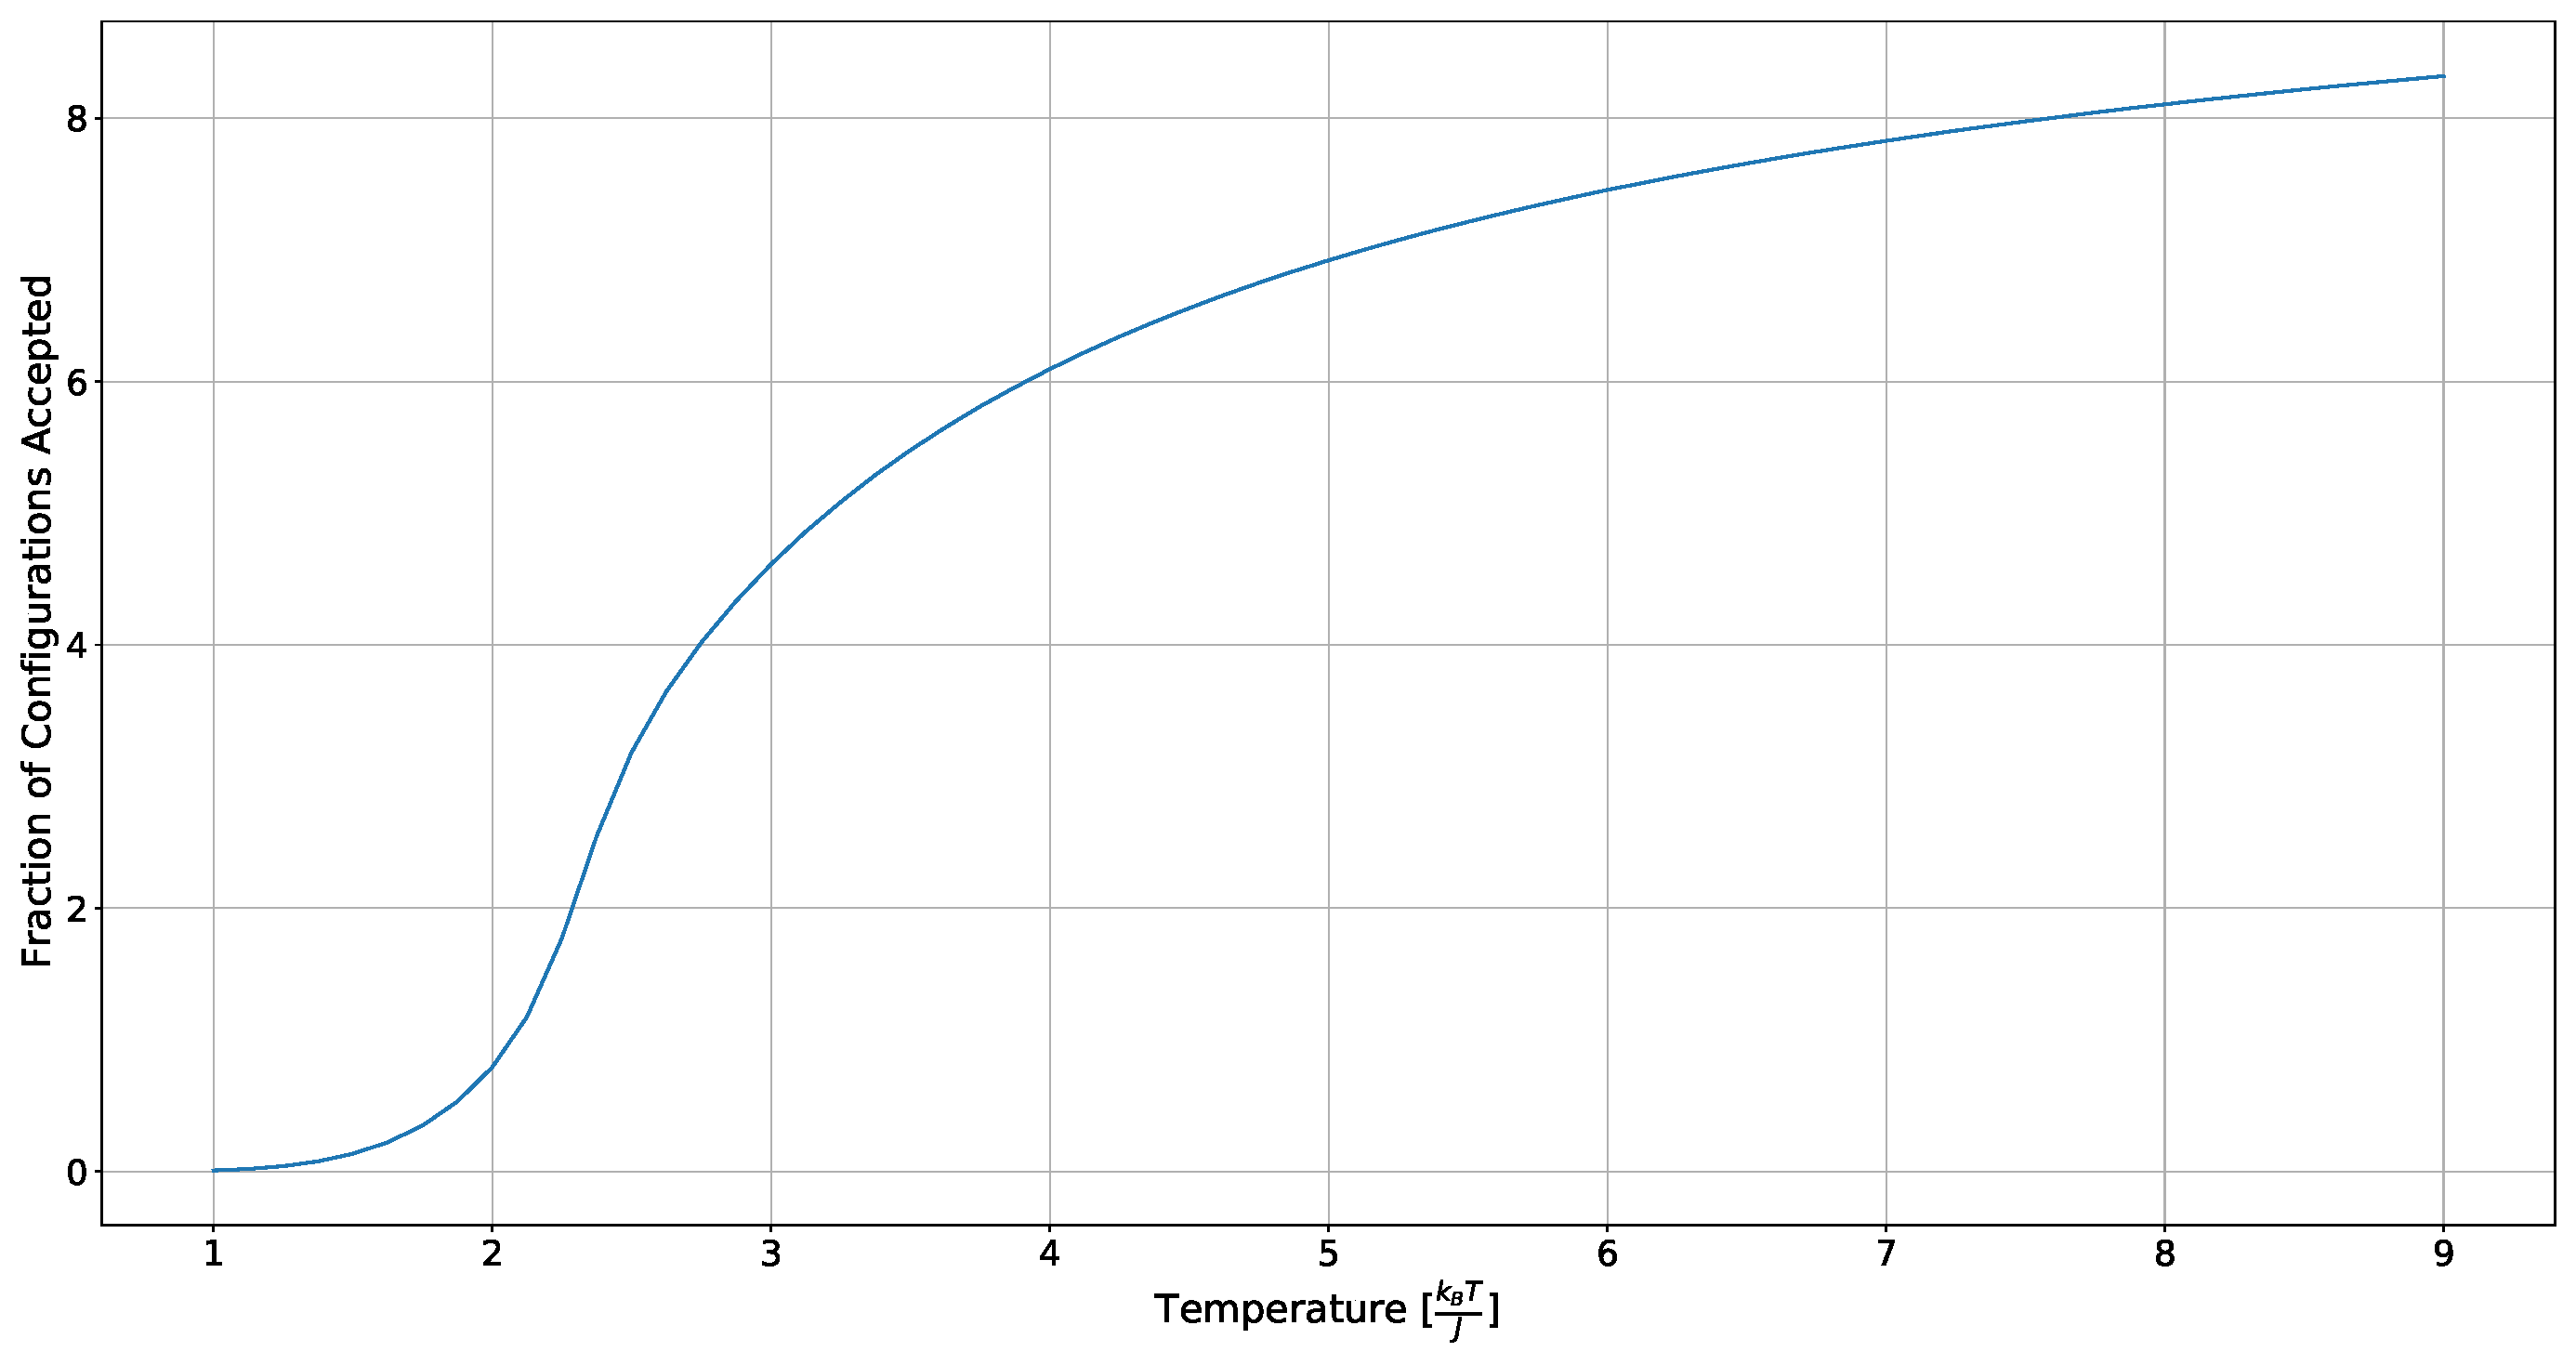
\includegraphics[trim=0.cm 0.cm 0.cm 0.cm, clip,width=1.0\textwidth]{../figures/config_ising_20x20_1E6_cycles_T_1.0_9.0_rng_1.pdf}
    \caption{Fraction of accepted spin-flips as a function of temperature, for $10^6$ MC cycles. The beginning state was randomized, and the resolution of the temperature is $0.125$}
    \label{fig:spin-flips-temp}
\end{figure}

\newpage

\subsection{Probability distribution function}

We find the probability for the system to be in each state according to the simulation after equilibration time for select temperatures.

\begin{figure}[htb!]
    \centering
    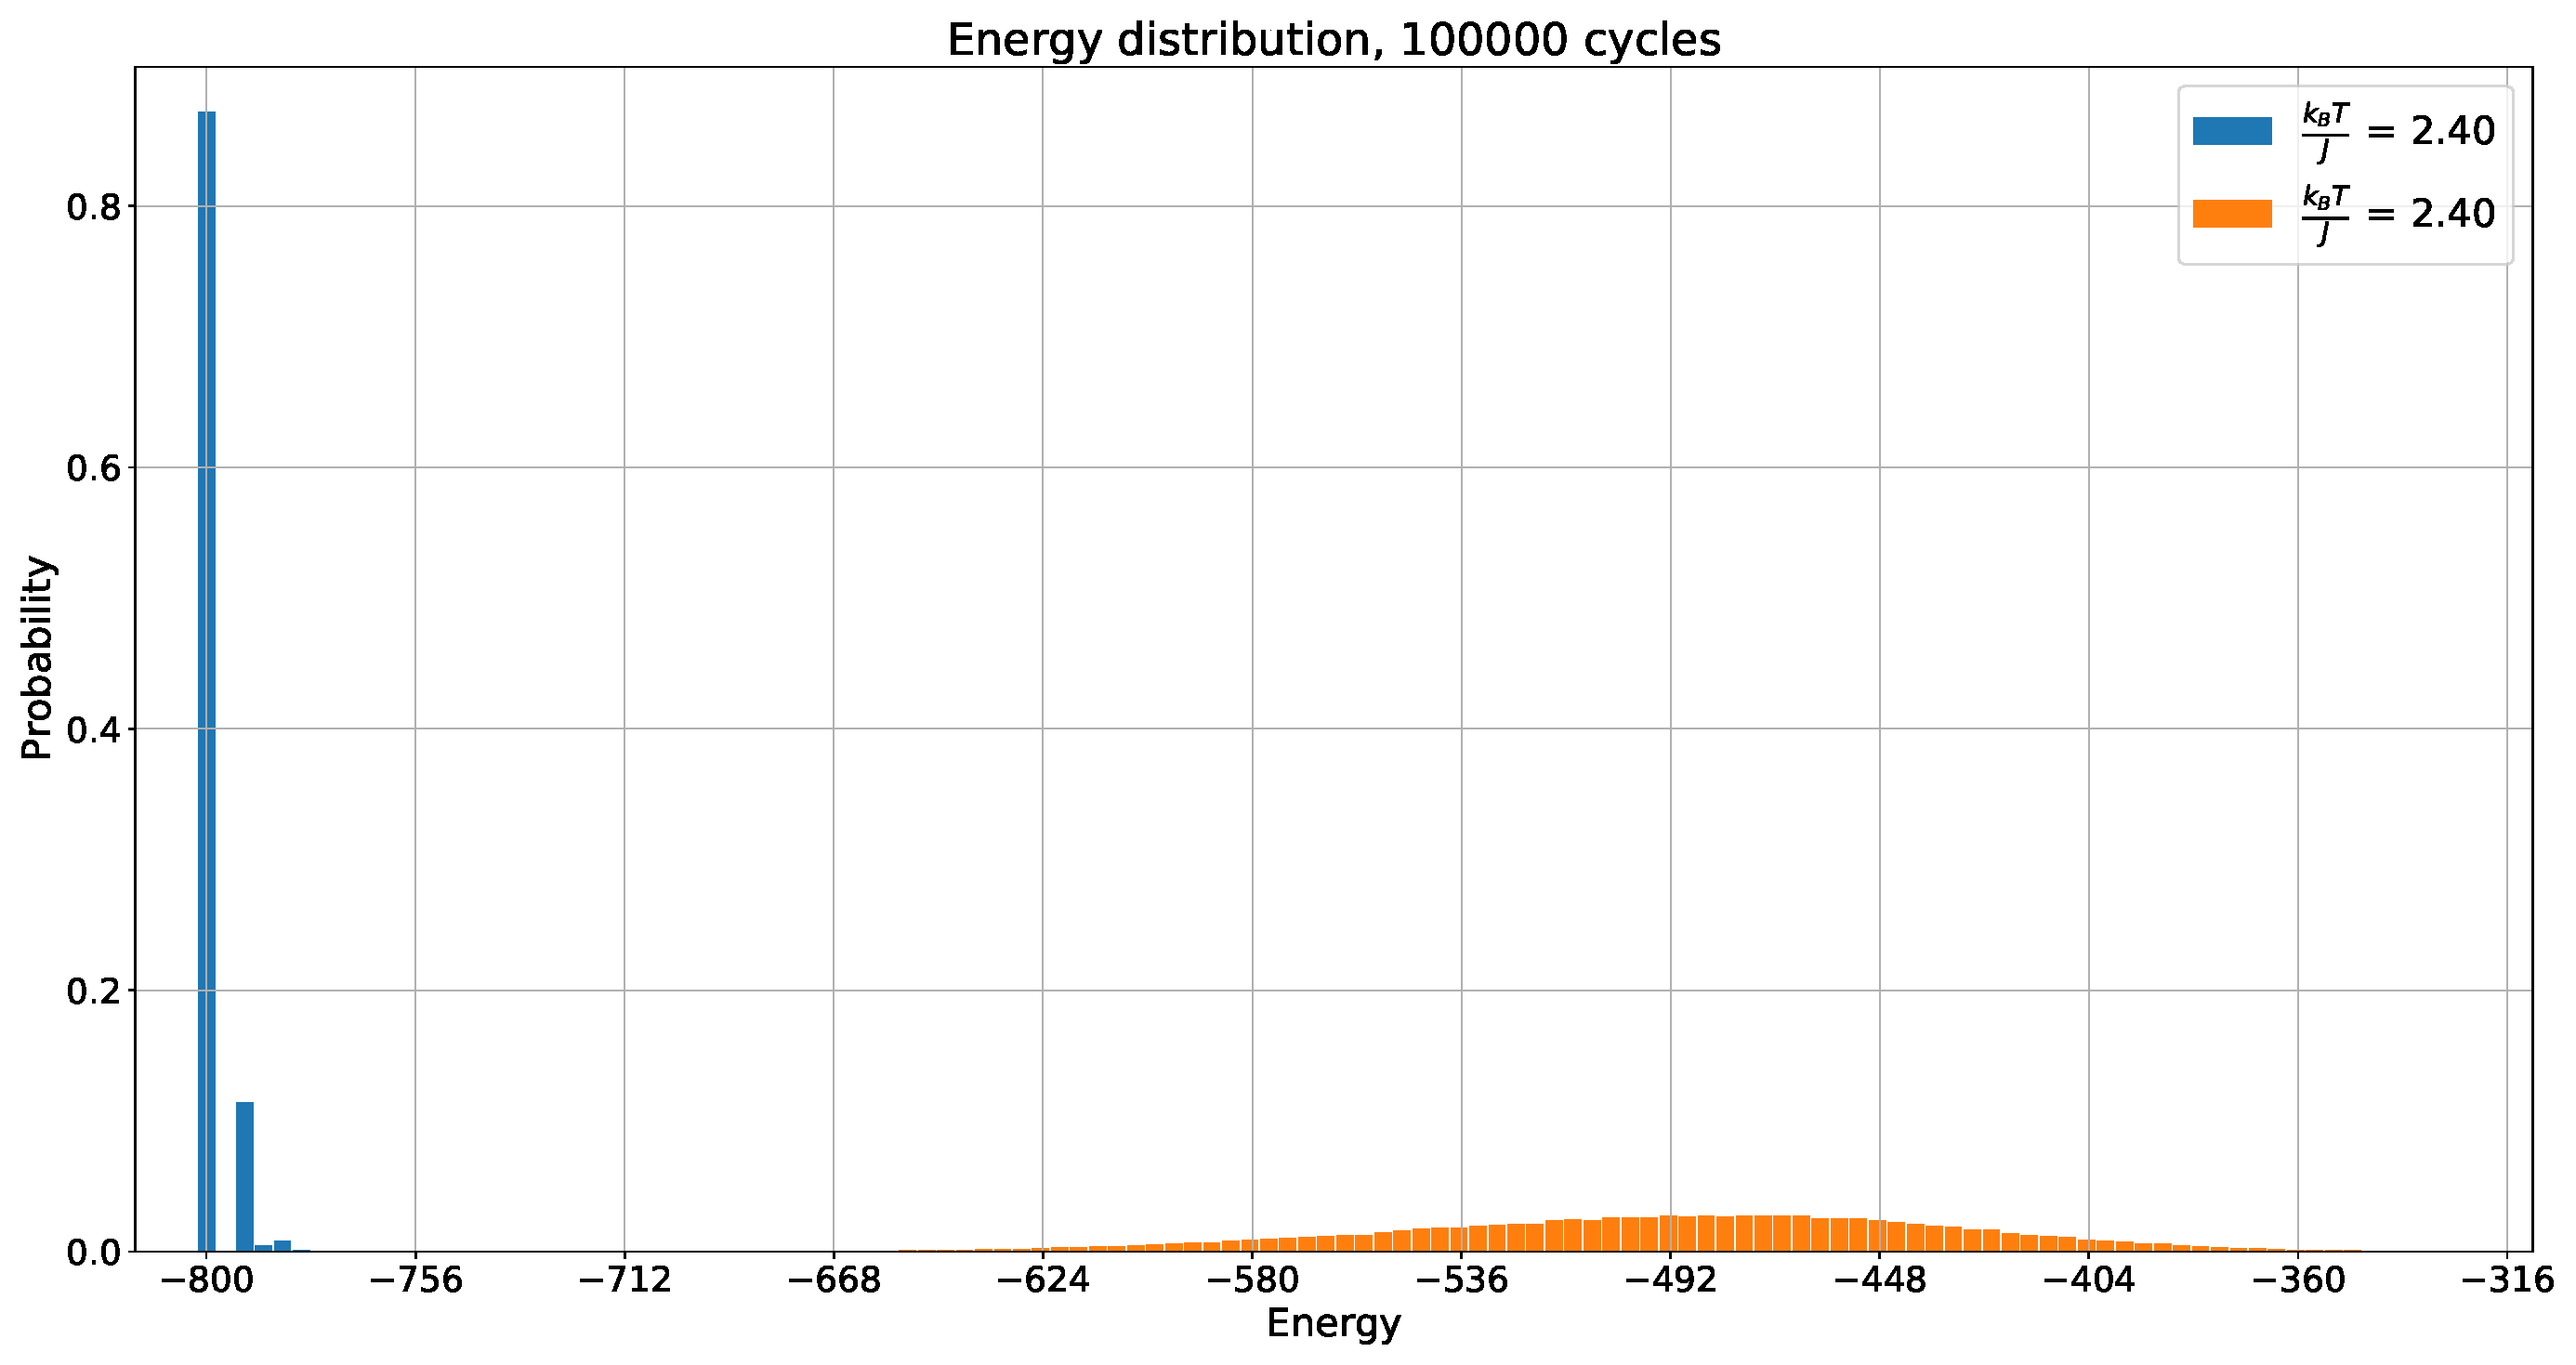
\includegraphics[trim=0.cm 0.cm 0.cm 1.15cm, clip,width=1.0\textwidth]{../figures/distribution_ising_20x20_1E5_cycles_T_1.0_2.4.pdf}
    \caption{Distribution of states plotted against the energy of each state. The system is a $20 \times 20$ lattice, for two temperatures $\frac{k_B T}{J} = \{1.0, 2.4\}$. There is a clear difference between the two temperatures, with the $k_B T = 1.0$ case being in the ground state more than 80\% of cycles, while the $k_B T = 2.4$ case being much more spread out around the $E = -492$ state. We have here used an equilibration time of $10\%$ of the MC cycles, or 1000 cycles, such that only the data after this number of cycles has passed is included.}
    \label{fig:energy-distribution}
\end{figure}


\subsection{Phase transition and critical temperature}

In \cref{fig:parallelisation} we plot the four thermodynamic values against temperature for four different lattice sizes, near the analytic critical temperature. This was done using parallellized code as the calculations are very time consuming. 

\begin{figure}[htb!]
    \centering
    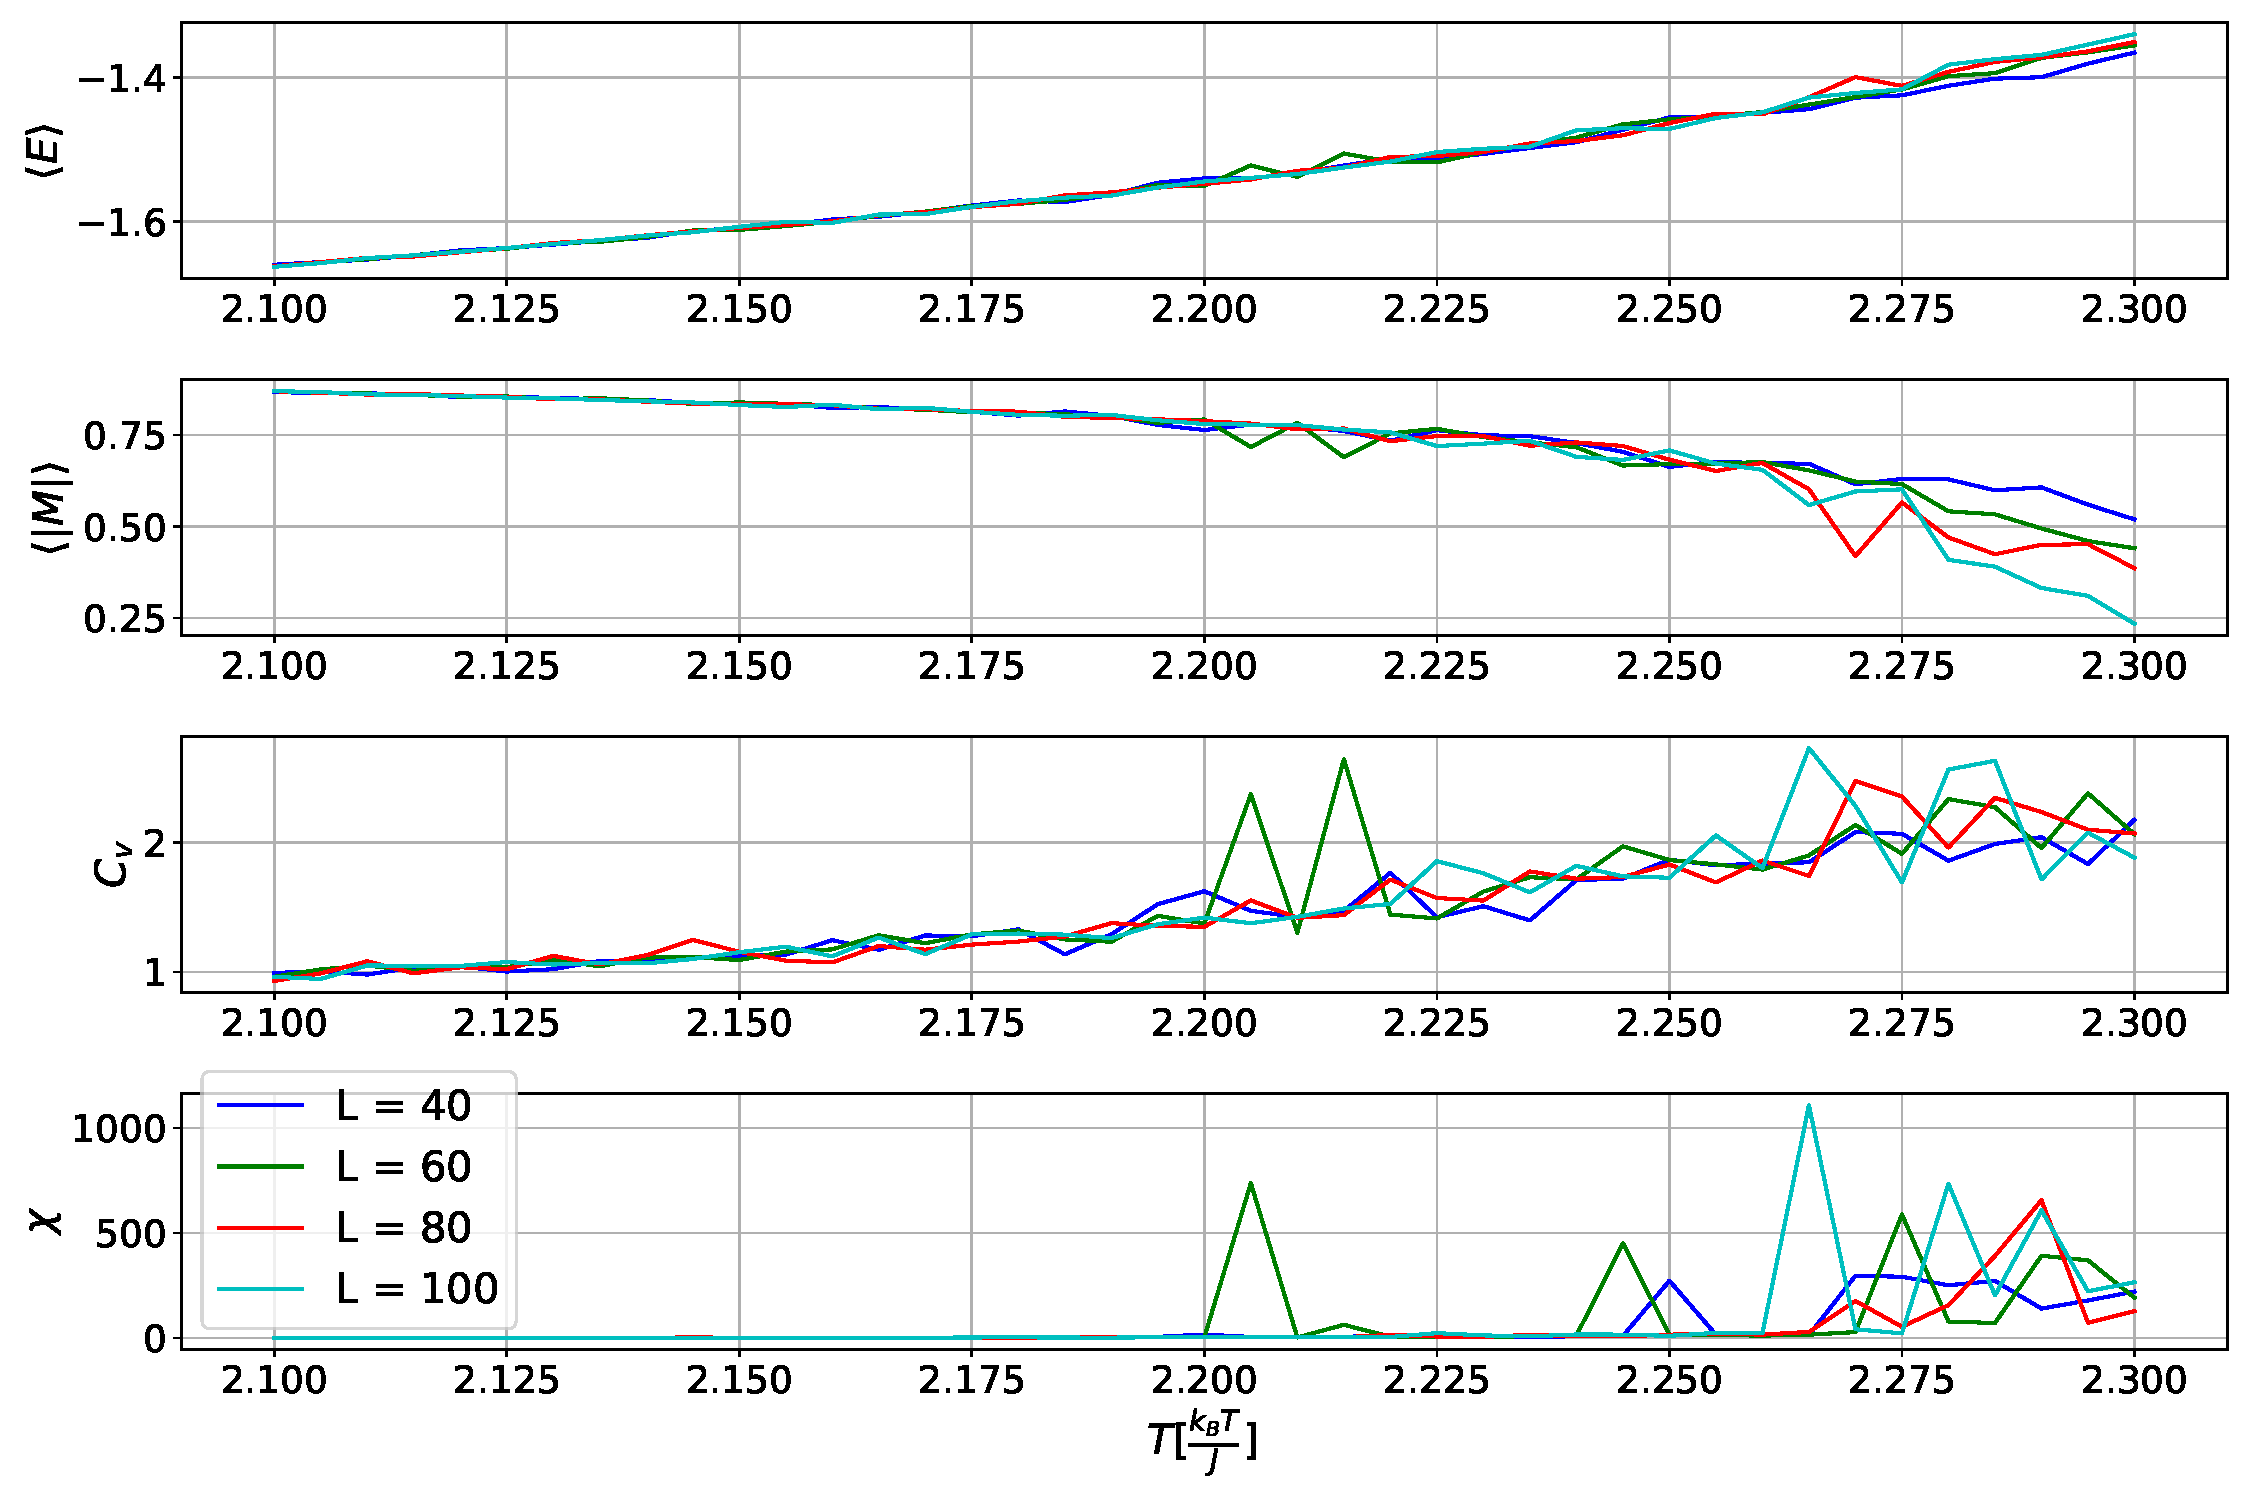
\includegraphics[trim=0.cm 0.cm 0.cm 0.cm, clip,width=1.0\textwidth]{../figures/mpi_values.pdf}
    \caption{Behavior of the Ising model in two dimensions close to the critical temperature for different lattice sizes $L$. Comparison of the expectation values for energy $\left\langle E \right\rangle$ and the absolute magnetization $\left\langle |M| \right\rangle$, the specific heat $C_v$ and the magnetic susceptibility $\chi$ for temperatures in the range $T \in [2.0, 2.3]$ with $\Delta T = 0.005$. There was done a total of $1\text{E}6$ cycles per value of $\Delta T$. All values are defined to be unit-less. Note that we have here cut off part of the plot to focus more on the interesting areas.}
    \label{fig:parallelisation}
\end{figure}
\newpage


\begin{table}[!htb]
\caption{Comparison of time elapsed in seconds before completion of simulation with and without running tasks in parallel. $t$ is time taken without adding parallelization to our code and $t_p$ is with. } 
\begin{center}
\begin{tabular}{ c c c }
\toprule
$L$ & $t[\text{s}]$ & $t_{p}[\text{s}$] \\

\midrule
$40$ & 3295 & 1624\\
$60$ & 7302 & 3534\\
$80$ &  12336 & 6071 \\
$100$ &  19328 & 9213\\


\midrule
\end{tabular}
\end{center}
\label{tab:timing}
\end{table}


In table [\ref{tab:timing}] we compare the time taken to complete the simulations done in figure [\ref{fig:parallelisation}], but using $\Delta T = 0.01$ instead. 
\end{document}
